% with xelatex
\documentclass[border=1pt]{standalone}

%\usepackage[utf8]{inputenc}
%\usepackage[T1]{fontenc}

%\usepackage{upgreek}
%\usepackage{arev}
%\usepackage{helvet}
%\usepackage{graphicx}
\usepackage{tikz}
\usepackage{tkz-euclide}
%\usepackage{pst-solides3d}
%\usepackage{auto-pst-pdf}
\usetikzlibrary{calc,decorations.pathmorphing,shapes,backgrounds,arrows.meta,arrows,automata,positioning}

%\renewcommand{\familydefault}{\sfdefault}

\usepackage{mathspec}
%\setallmainfonts{Linux Libertine O}
\setallmainfonts{Arial}

\begin{document}

  \begin{tikzpicture}
    \node at (0,0) {
\includegraphics[scale=0.8]{wals}};
    \node at (-4.6,3.2) {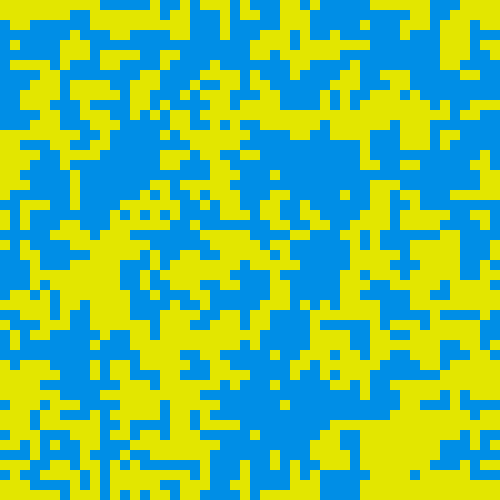
\includegraphics[width=2cm]{snapshot1}};
    \draw (-5.6,4.2) rectangle (-3.6,2.2);
    \draw (-4.6,2.2) -- (-3.08,0.02);
    \node at (-1.5,3.2) {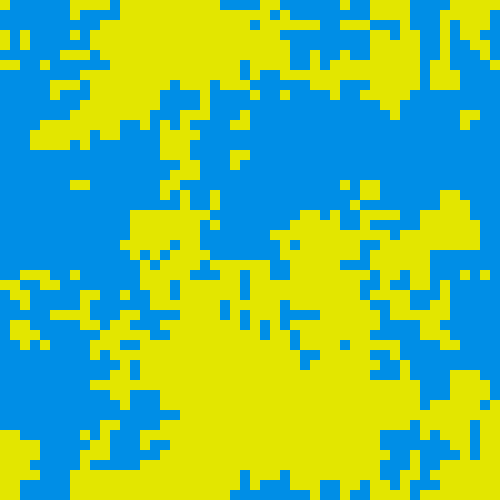
\includegraphics[width=2cm]{snapshot2}};
    \draw (-2.5,4.2) rectangle (-0.5,2.2);
    \draw (-1.5,2.2) -- (-3.06,-1.07);
    \node at (-3.0,-6.0) {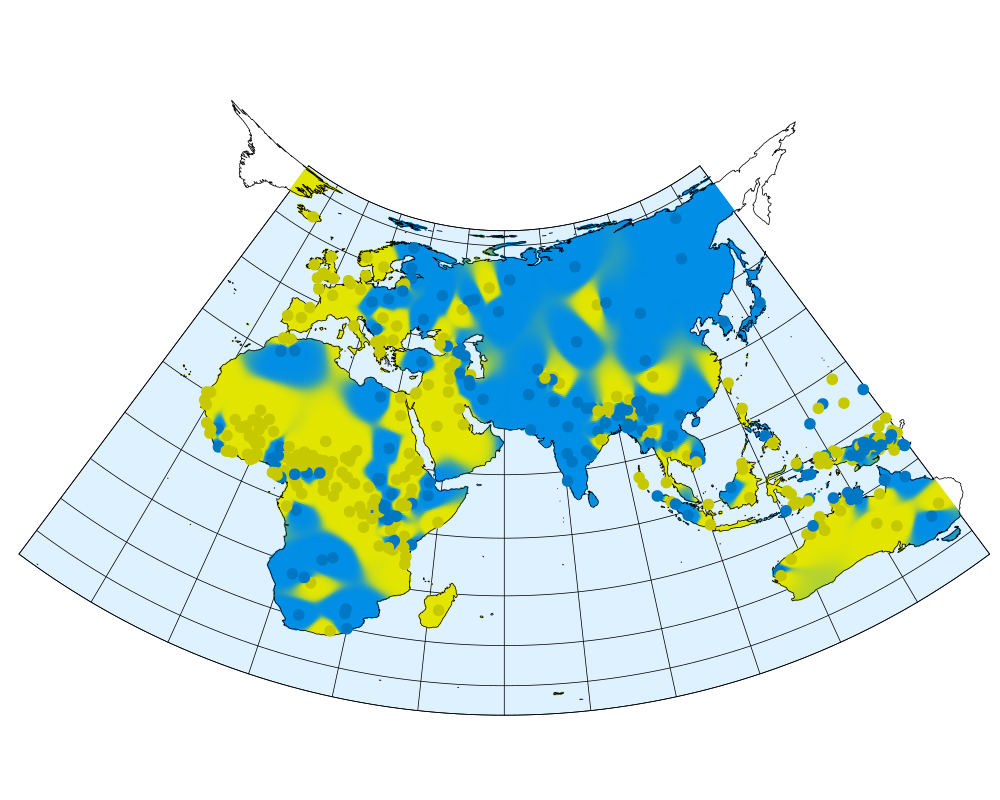
\includegraphics[scale=0.17]{interp_1}};
    \node at (4.0,-6.0) {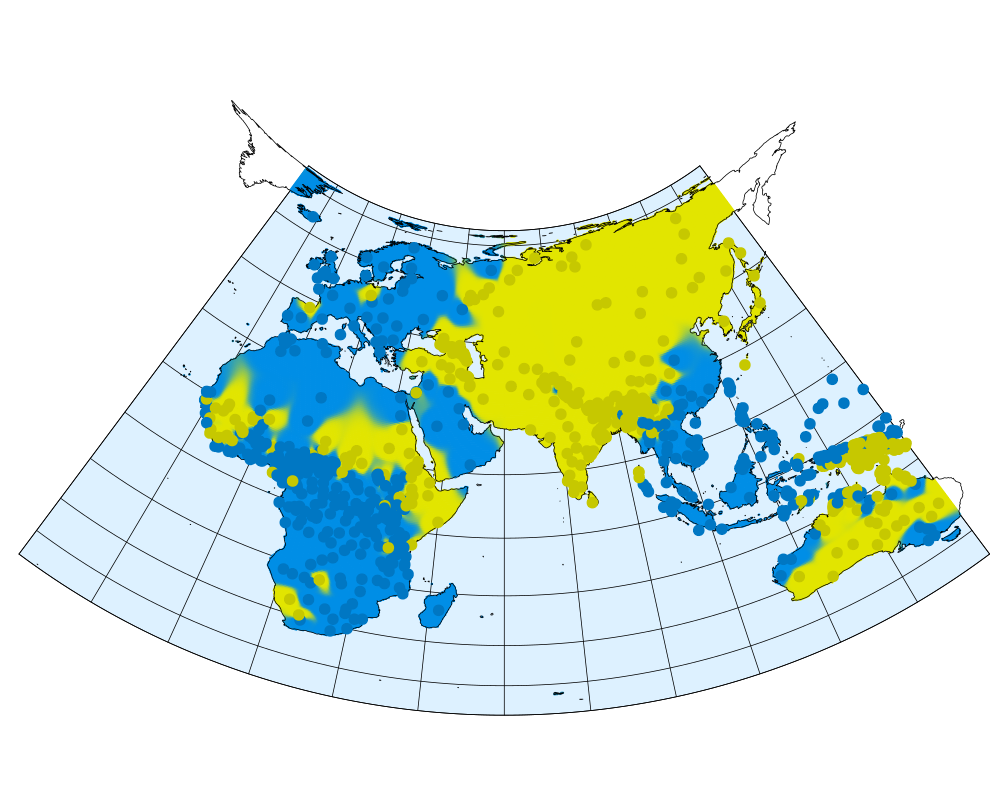
\includegraphics[scale=0.17]{interp_2}};
    \node at (-5.0,1.2) [above] {\textbf{a}};
    \node at (2.1,1.2) [above] {\textbf{b}};
    \node at (-5.0,-4.4) [above] {\textbf{c}};
    \node at (2.1,-4.4) [above] {\textbf{d}};
  \end{tikzpicture}

\end{document}
